\documentclass[11pt,a4paper]{article}

\usepackage[margin=2.4cm]{geometry}
\usepackage[T1]{fontenc}
\usepackage{lmodern}
\usepackage{amsmath,amssymb}
\usepackage{graphicx}
\usepackage{booktabs}
\usepackage{xcolor}
\usepackage{tcolorbox}
\usepackage{listings}
\usepackage{caption}
\usepackage[hidelinks]{hyperref}

\definecolor{accent}{HTML}{2E6FDB}
\definecolor{warn}{HTML}{D1495B}
\definecolor{soft}{HTML}{F2F5FB}

\lstset{
  basicstyle=\ttfamily\footnotesize,
  backgroundcolor=\color{soft},
  frame=single, rulecolor=\color{gray!40},
  breaklines=true, showstringspaces=false,
  columns=fullflexible, xleftmargin=0pt, framexleftmargin=3pt,
}

\captionsetup{font=small, labelfont={bf,color=accent}}

\newcommand{\ADU}{\ensuremath{\mathrm{ADU}}}
\newcommand{\eminus}{\ensuremath{\mathrm{e}^-}}

\title{\vspace{-1.5cm}\textbf{Optimal histogram binning for EMCCD\\photon-counting flux retrieval}}
\author{\normalsize How many bins, and exactly where to cut}
\date{\normalsize Generated by \texttt{bin\_optimizer.py} and \texttt{demo\_optimal\_bins.py}\\
\normalsize \today}

\begin{document}
\maketitle
\vspace{-0.8cm}

\begin{tcolorbox}[colback=soft,colframe=accent,title=\textbf{Answer in one box}]
For an EMCCD read out with bias $b$, mean EM gain $G$, read noise $\sigma$ and
saturation at $x_{\rm sat}$, working over $\mu \le 8\ \eminus$ per read:

\medskip
\textbf{Eight bins are enough.} They retain $\ge 98.3\,\%$ of the accuracy of
the full, undegraded 1\,\ADU\ histogram at every flux from $10^{-3}$ to
$8\ \eminus$/read. Four bins do not (89.5\,\%); eight is the smallest power of
two that clears the 95\,\% target, with margin.

\medskip
\textbf{Where the cuts go.} Write the pixel value in gain units,
$u = (x-b)/G$, and let $S = (x_{\rm sat}-b)/G$.

\begin{enumerate}\itemsep2pt
\item One cut just above the read-noise peak, at $x = b + c_1\sigma$ with
      $c_1 \simeq 4$ to $4.5$. This one number does almost all the work at low
      flux.
\item Six rungs spaced \emph{uniformly in} $\sqrt{u}$, from $u_1 \simeq 1$
      (one electron) up to
      $u_{\rm top} = \min\!\big(S,\ \mu_{\max} + 3\sqrt{\mu_{\max}}\big)$.
\item One open bin above $u_{\rm top}$, absorbing saturation and overflow.
\end{enumerate}

\medskip
The wide bin between cut 1 and $u_1$ is the single-electron shoulder and is
deliberately left unsplit.
\end{tcolorbox}

\section{The question, and what ``95\,\% of the accuracy'' means}

An EMCCD flux estimator that never stores the frames keeps, for each pixel, a
histogram of that pixel's raw \ADU\ values across all reads, and fits the mean
flux $\mu$ from that histogram. The histogram is the entire memory footprint of
the method, so its number of bins $K$ is the parameter that matters. The
question is how small $K$ can be before the flux estimate measurably degrades,
and where the $K$ bin edges belong.

The detector digitises to whole \ADU, so there is a natural, finite reference:
the \emph{full histogram}, one bin per \ADU,
\begin{equation}
  \text{cell } i = [i,\,i+1) \ \ \text{for } i < x_{\rm sat},
  \qquad
  \text{cell } x_{\rm sat} = [x_{\rm sat},\,\infty),
\end{equation}
the last cell holding everything that saturates, since saturated pixels are
mutually indistinguishable. Any $K$-bin histogram is a merge of contiguous runs
of these cells. By the data-processing inequality it can therefore never carry
\emph{more} information than the full histogram, which makes the comparison
below a clean, bounded one.

The relevant measure is the Fisher information about $\mu$ carried by one read
of one pixel,
\begin{equation}
  I(\mu) \;=\; \sum_{\text{bins } i} \frac{1}{p_i(\mu)}
                \left(\frac{\partial p_i}{\partial \mu}\right)^{2},
  \label{eq:fisher}
\end{equation}
with $p_i(\mu)$ the probability that a read lands in bin $i$. Over $N$ reads the
Cram\'er-Rao bound gives $\sigma_{\hat\mu} = 1/\sqrt{N I(\mu)}$, so the
comparison between a $K$-bin design and the full histogram is
\begin{equation}
  \boxed{\;
  \eta(\mu) \;=\; \frac{I_K(\mu)}{I_{\rm full}(\mu)},
  \qquad
  \frac{\sigma_{\rm full}}{\sigma_K} \;=\; \sqrt{\eta(\mu)}\;}
  \label{eq:eta}
\end{equation}
We call $\eta$ the \emph{information efficiency} and $\sqrt{\eta}$ the
\emph{accuracy retained}. ``Recovering more than 95\,\% of the accuracy'' is
read literally as $\sqrt{\eta} \ge 0.95$ at every flux in the range of
interest, i.e. $\eta \ge 0.9025$. Both numbers are quoted throughout, because
the stricter reading $\eta \ge 0.95$ is also of interest and the eight-bin
design happens to satisfy it too.

Two properties of \eqref{eq:fisher} drive everything that follows. It is a
\emph{sum over bins}, which makes the optimisation exactly solvable
(Section~\ref{sec:opt}); and it is bounded above by the full-histogram value,
which makes $\eta \le 1$ by construction.

\section{The signal chain, and its two dimensionless numbers}

One read of one pixel is
\begin{equation}
  n \sim \mathrm{Poisson}(\mu + \mu_{\rm CIC}),
  \qquad
  g \sim \mathrm{Gamma}(n, G) \ \ (g=0 \text{ if } n=0),
  \qquad
  x = b + g + \mathcal{N}(0,\sigma^2),
\end{equation}
truncated at $x_{\rm sat}$. The zero-electron case is a pure Gaussian at the
bias; each additional electron adds one more Gamma stage of mean $G$. This is
the standard EMCCD model of Basden et al. (2003), as used by Harps{\o}e et al.
(2012) and Daigle et al. (2009).

Rescaling by the gain removes all but two free numbers:
\begin{equation}
  u = \frac{x-b}{G},
  \qquad
  r = \frac{\sigma}{G} \ \ \text{(read noise in gain units)},
  \qquad
  S = \frac{x_{\rm sat}-b}{G} \ \ \text{(saturation head-room)}.
\end{equation}
The optimal design depends on the detector only through $r$ and $S$, and on the
science only through the flux range $[\mu_{\min}, \mu_{\max}]$. The worked
example throughout is $b=1000$, $G=5000\ \ADU/\eminus$, $\sigma=30\ \ADU$,
$x_{\rm sat}=60000\ \ADU$, $\mu_{\rm CIC}=10^{-3}$, giving $r = 0.0060$ and
$S = 11.8\ \eminus$. A second detector with a much larger $r$ is treated in
Section~\ref{sec:pesto}.

\section{Where the flux information actually sits}
\label{sec:physics}

Before optimising anything, it pays to see what the answer must look like.
Figure~\ref{fig:cuts} shows the pixel-value distribution and the Fisher
information density, split into the read-noise peak (left, in units of $\sigma$)
and the EM tail (right, in units of $G$). These are two utterly different
scales: the peak is $\sim\!10^{-2}$ wide in $u$, the tail is $\sim\!10$ wide.

\begin{figure}[t]
\centering
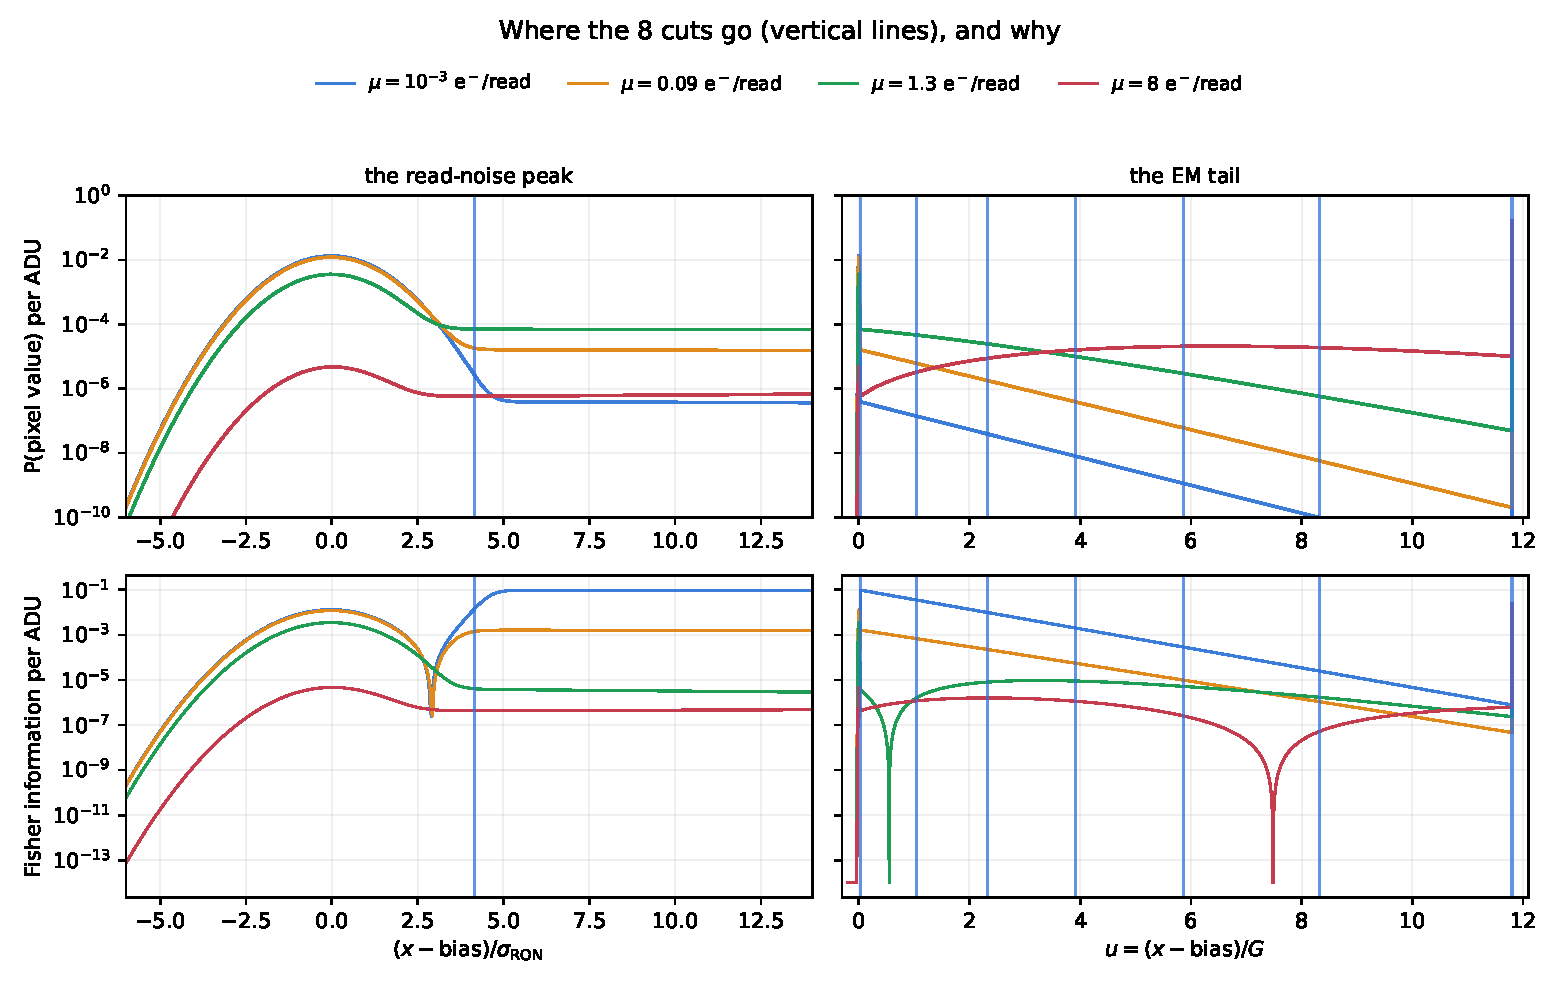
\includegraphics[width=\textwidth]{figures/bins/fig2_where_the_cuts_go.pdf}
\caption{The eight cuts (vertical lines) against the distribution they bin.
Left: the read-noise peak, in units of the read noise. Right: the EM tail, in
units of the gain. Top: the pixel-value probability per \ADU. Bottom: the Fisher
information about $\mu$ per \ADU. A single cut at $+4.2\sigma$ serves the whole
peak; the remaining cuts climb the tail. The dips in the bottom panels are
where $\partial p/\partial\mu$ changes sign, not zeros of the density.}
\label{fig:cuts}
\end{figure}

\subsection{Low flux: the histogram collapses to a single threshold}

Consider $\mu \to 0$, so that reads are almost all $n=0$ with an occasional
$n=1$. Put the first cut at $u_1$, and suppose the read noise leaks negligibly
above it. Then every bin $j$ lying above the cut contains only single-electron
events, so $p_j = \lambda g_j$ and $\partial p_j/\partial\mu = g_j$, where
$g_j$ is the $n=1$ mass in that bin and $\lambda = \mu + \mu_{\rm CIC}$. Its
contribution to \eqref{eq:fisher} is
\begin{equation}
  \frac{(\partial p_j/\partial\mu)^2}{p_j} \;=\; \frac{g_j}{\lambda},
  \qquad\text{so}\qquad
  \sum_{j \,\text{above the cut}} \frac{g_j}{\lambda}
  \;=\; \frac{e^{-u_1}}{\lambda}.
  \label{eq:telescope}
\end{equation}
The sum \emph{telescopes}. It depends on where the first cut is and on nothing
else: how the region above the cut is subdivided is irrelevant. At low flux the
histogram is worth exactly as much as a single threshold.

That is not a heuristic, and Table~\ref{tab:telescope} confirms it numerically.
Two bins, meaning one threshold, already match the full eight-bin design below
$\mu \sim 10^{-2}\ \eminus$/read. Bins only begin to earn their keep as $\mu$
approaches one electron per read, when double and triple electrons populate the
tail and its \emph{shape}, not just its total, starts to carry information.

\begin{table}[h]
\centering
\small
\caption{Information efficiency $\eta$ of designs sharing the same first cut
(1125\,\ADU) but differing in how many bins sit above it. At low flux the extra
bins buy nothing, exactly as \eqref{eq:telescope} predicts.}
\label{tab:telescope}
\begin{tabular}{lccccc}
\toprule
& \multicolumn{5}{c}{$\mu$ [\eminus/read]}\\
\cmidrule(l){2-6}
design & $10^{-3}$ & $10^{-2}$ & $10^{-1}$ & $1$ & $8$\\
\midrule
2 bins (one threshold) & 0.9944 & 0.9985 & 0.9940 & 0.8199 & 0.0062\\
3 bins                 & 0.9944 & 0.9985 & 0.9948 & 0.8983 & 0.4411\\
8 bins, optimal        & 0.9945 & 0.9985 & 0.9963 & 0.9827 & 0.9678\\
\bottomrule
\end{tabular}
\end{table}

\subsection{The first cut: a tension between two leaks}
\label{sec:firstcut}

Equation~\eqref{eq:telescope} assumed the read noise does not leak above the
cut. That assumption is the single most important design constraint, and
getting it wrong is catastrophic rather than merely suboptimal. If a fraction
$Q(c_1) = \tfrac12\,\mathrm{erfc}(c_1/\sqrt2)$ of the zero-electron peak sits
above a cut at $b + c_1\sigma$, then the bin just above the cut contains a
flux-independent population $Q$ alongside the flux-carrying population
$\sim\!\lambda$. Its contribution stops scaling as $1/\lambda$ and saturates at
$O(1)$: the information is gone.

So $c_1$ is squeezed from both sides:
\begin{align}
  \text{from below:}\quad & Q(c_1) \ll \mu_{\min}
    && \text{or the peak's own tail swamps the electrons;}\\
  \text{from above:}\quad & 1 - e^{-c_1 r} \ll 1
    && \text{since that fraction of single electrons falls into bin 0.}
\end{align}
Table~\ref{tab:firstcut} evaluates both. For the worked detector, $c_1 = 4$ to
$4.5$ is comfortable: the leak is $10^{-5}$ or below, well under
$\mu_{\min}=10^{-3}$, while only $2.4$ to $2.7\,\%$ of single electrons are
sacrificed. The numerical optimum lands at $c_1 = 4.17$, which is simply where
these two curves cross.

This is also where the user's intuition about ``a few sigma'' is made precise:
the right number of sigmas is $c_1 \simeq Q^{-1}(\mu_{\min})$, so a lower
target flux pushes the cut outward, logarithmically slowly.

\begin{table}[h]
\centering
\small
\caption{The two competing leaks as a function of the first cut position
$c_1$, for the worked detector ($r=0.0060$) and for a detector with much
larger read noise relative to gain ($r=0.0959$, Section~\ref{sec:pesto}).
The optimum sits where the read-noise leak has become negligible but the
electron loss has not yet become expensive.}
\label{tab:firstcut}
\setlength{\tabcolsep}{4pt}
\begin{tabular}{lcccccc}
\toprule
$c_1$ [$\sigma$] & 2.0 & 3.0 & 3.5 & 4.0 & 4.5 & 5.0\\
\midrule
read-noise leak $Q(c_1)$ & $2.3{\cdot}10^{-2}$ & $1.4{\cdot}10^{-3}$ & $2.3{\cdot}10^{-4}$ & $3.2{\cdot}10^{-5}$ & $3.4{\cdot}10^{-6}$ & $2.9{\cdot}10^{-7}$\\
electrons lost, $r=0.0060$ & 1.19\,\% & 1.78\,\% & 2.08\,\% & 2.37\,\% & 2.66\,\% & 2.96\,\%\\
electrons lost, $r=0.0959$ & 17.5\,\% & 25.0\,\% & 28.5\,\% & 31.9\,\% & 35.0\,\% & 38.1\,\%\\
\bottomrule
\end{tabular}
\end{table}

\subsection{The tail: uniform in $\sqrt{u}$}

Above the peak the distribution is a Poisson mixture of Gamma laws. The
$n$-electron component has mean $nG$ and standard deviation $\sqrt{n}\,G$, so at
a pixel value $u$ the local width of the structure that must be resolved grows
like $\sqrt{u}$. Bins whose widths follow that growth, i.e. rungs placed
uniformly in $\sqrt{u}$, keep a constant number of bins per local width
everywhere along the tail. Formally, $\sqrt{u}$ is the variance-stabilising
transform of the Gamma family, the same argument that puts $\sqrt{\cdot}$ at the
heart of Anscombe-type transforms.

The numerical optimum reproduces this without being told. For the eight-bin
design the successive rungs sit at
\begin{equation*}
  \sqrt{u} \;=\; 1.02,\quad 1.52,\quad 1.98,\quad 2.42,\quad 2.88,\quad 3.44,
\end{equation*}
with increments $0.51$, $0.46$, $0.44$, $0.46$, $0.55$: uniform to within a few
percent, over a range in $u$ itself spanning more than a factor of ten.
Restricting the closed-form family of Section~\ref{sec:opt} to one ladder shape
at a time and re-optimising every other parameter gives worst-case
$\eta = 0.9643$ for $\sqrt{u}$, $0.9594$ for $\log u$ and $0.9480$ for $u$
itself. The log-uniform ladder, the natural first guess, is the runner-up
rather than a disaster; it over-resolves the region just above the peak, where
\eqref{eq:telescope} has already shown there is nothing to resolve, and pays
for it at the top of the range.

\subsection{The top cut: stop where the counts stop}

The last finite edge should not be placed at saturation out of habit. Bins
placed where no read ever lands are wasted. Since the pixel value of an
$n$-electron event is $\sim\!n \pm \sqrt{n}$ in gain units, and $n$ itself
rarely exceeds $\mu + 3\sqrt{\mu}$,
\begin{equation}
  u_{\rm top} \;=\; \min\!\Big(S,\ \ \mu_{\max} + 3\sqrt{\mu_{\max}}\Big).
\end{equation}
For the worked detector $S = 11.8$ is smaller than $8 + 3\sqrt{8} = 16.5$, so
real saturation binds and the top cut sits at $x_{\rm sat}$. For a detector
with generous head-room the second term binds instead, and the optimiser duly
places the top cut well below saturation (Section~\ref{sec:pesto}).

Figure~\ref{fig:cumul} closes the argument: it shows the cumulative fraction of
the flux information as a function of pixel value. The cuts are placed so that
each bin carries a comparable share of the information, which is what
maximising \eqref{eq:fisher} under a bin budget amounts to.

\begin{figure}[t]
\centering
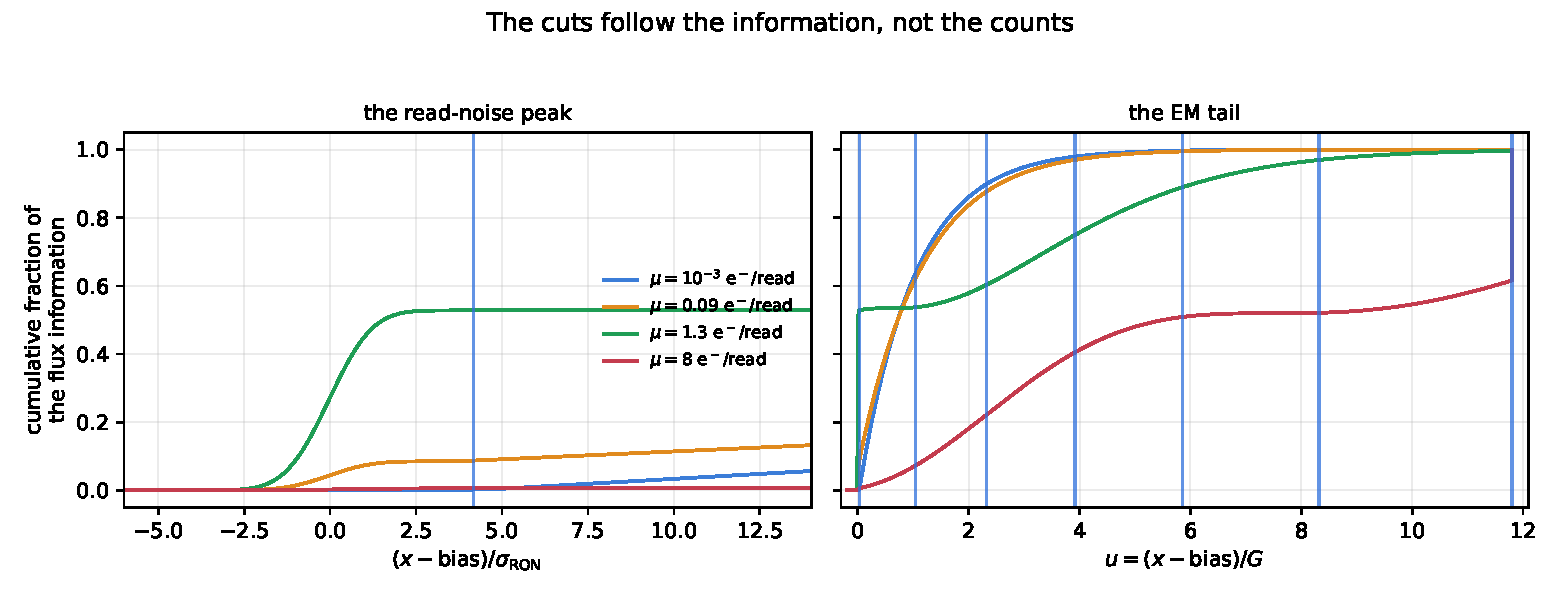
\includegraphics[width=\textwidth]{figures/bins/fig3_information.pdf}
\caption{Cumulative fraction of the flux information versus pixel value, at
four fluxes, with the eight cuts overlaid. At $\mu = 10^{-3}\ \eminus$/read
essentially all of the information is collected by the first cut. By
$\mu = 8\ \eminus$/read it is spread across the whole tail, which is why the
tail rungs exist.}
\label{fig:cumul}
\end{figure}

\section{Finding the optimum, not just a good guess}
\label{sec:opt}

Because \eqref{eq:fisher} is additive over bins, a weighted objective
\begin{equation}
  V \;=\; \sum_{\mu} w_\mu \, \frac{I_K(\mu)}{I_{\rm full}(\mu)}
     \;=\; \sum_{\text{bins } i} \underbrace{\left[
        \sum_\mu \frac{w_\mu}{I_{\rm full}(\mu)}\,
        \frac{(\Delta_i \partial_\mu P)^2}{\Delta_i P}\right]}_{\text{depends only on bin } i}
\end{equation}
is also additive over bins, where $\Delta_i$ denotes the difference of the
cumulative distribution across bin $i$. A contiguous partition with an additive
value admits an exact dynamic program: the best $K$-bin partition ending at a
given edge is built from the best $(K-1)$-bin partition ending at each earlier
edge. Restricted to a dense candidate set of edges (about 560 positions, spaced
$0.1\sigma$ through the peak and logarithmically above it), the optimum is
therefore \emph{global}, not the result of a local search.

The design must be good over a \emph{range} of fluxes, not at one flux, so what
is actually wanted is the max-min solution
$\max_{\rm edges} \min_\mu \eta(\mu)$. That is not additive, but it is the dual
of a weighted problem: a multiplicative-weights loop repeatedly solves the
additive problem exactly and then shifts $w_\mu$ towards whichever fluxes are
currently worst served. Forty rounds converge to within $10^{-3}$ in $\eta$ and
take under two seconds.

The result is a hard yardstick. A closed-form family that matches it is not
merely plausible, it is provably close to the best a $K$-bin histogram can do.
The three-zone family of the summary box recovers $99.9\,\%$ of the dynamic
programme's worst-case $\eta$ at $K=8$, and matches it at $K=16$.

\section{Results}

\subsection{How many bins}

\begin{table}[h]
\centering
\small
\caption{Worst-case performance over $\mu \in [10^{-3},\,8]\ \eminus$/read, for
the worked detector. ``Accuracy'' is $\sigma_{\rm full}/\sigma_K = \sqrt{\eta}$,
the quantity the 95\,\% target applies to. The last column is what $K$
equal-width bins from bias to saturation would give.}
\label{tab:kscan}
\begin{tabular}{rccc c}
\toprule
$K$ & $\eta$ (worst) & accuracy & meets 95\,\%? & equal-width accuracy\\
\midrule
 4 & 0.8015 & 89.5\,\% & no  & 14.3\,\%\\
 5 & 0.8859 & 94.1\,\% & no  & 23.4\,\%\\
 6 & 0.9284 & 96.4\,\% & yes & 31.5\,\%\\
 7 & 0.9521 & 97.6\,\% & yes & 38.3\,\%\\
\textbf{8} & \textbf{0.9657} & \textbf{98.3\,\%} & \textbf{yes} & 44.1\,\%\\
12 & 0.9872 & 99.4\,\% & yes & 59.8\,\%\\
16 & 0.9928 & 99.6\,\% & yes & 69.0\,\%\\
32 & 0.9982 & 99.9\,\% & yes & 78.4\,\%\\
\bottomrule
\end{tabular}
\end{table}

Table~\ref{tab:kscan} and Figure~\ref{fig:kscan} give the headline result.
Eight bins is the smallest power of two that meets the target, and it does so
with room to spare: $98.3\,\%$ of the full-histogram accuracy in the worst case,
against a $95\,\%$ requirement. Six bins would also pass, but eight is both a
power of two and noticeably safer. Four bins fall short at $89.5\,\%$.

The equal-width column is worth dwelling on. Spreading $K$ bins uniformly from
bias to saturation, the obvious thing to do without thinking about it, gives
$44\,\%$ at $K=8$ and still only $78\,\%$ at $K=32$: it never catches up,
because it spends essentially all of its bins on the empty region above the
signal and none on the read-noise peak, where at low flux all of the information
is. The gain from thinking about bin placement is far larger than the gain from
quadrupling the number of bins.

\begin{figure}[t]
\centering
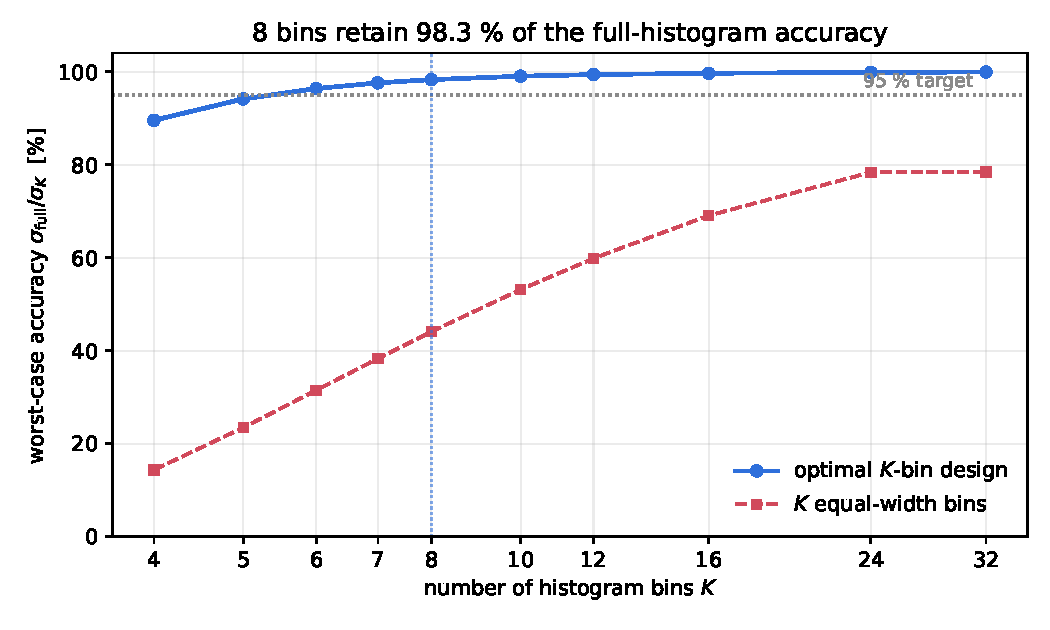
\includegraphics[width=0.85\textwidth]{figures/bins/fig1_bin_count.pdf}
\caption{Worst-case accuracy retained versus the number of bins, over
$\mu \in [10^{-3},\,8]\ \eminus$/read. The optimised design saturates quickly;
equal-width bins never recover.}
\label{fig:kscan}
\end{figure}

\subsection{The eight-bin design, cut by cut}

\begin{table}[h]
\centering
\small
\caption{The eight-bin design for $b=1000$, $G=5000\ \ADU/\eminus$,
$\sigma=30\ \ADU$, $x_{\rm sat}=60000\ \ADU$, optimised over
$\mu \in [10^{-3},\,8]\ \eminus$/read. Bin~0 absorbs everything below the first
cut, bin~7 everything above the last. The rightmost column shows the cut
positions in $\sqrt{u}$, whose near-constant spacing above $u_1$ is the
signature discussed in Section~\ref{sec:physics}.}
\label{tab:design8}
\begin{tabular}{rrrrrr}
\toprule
bin & lower [\ADU] & upper [\ADU] & $u_{\rm lo}$ & $u_{\rm hi}$ & $\sqrt{u_{\rm hi}}$\\
\midrule
0 &     0 &  1\,125 & $-0.200$ &  0.025 & 0.16\\
1 & 1\,125 &  6\,176 &  0.025 &  1.035 & 1.02\\
2 & 6\,176 & 12\,596 &  1.035 &  2.319 & 1.52\\
3 & 12\,596 & 20\,591 &  2.319 &  3.918 & 1.98\\
4 & 20\,591 & 30\,324 &  3.918 &  5.865 & 2.42\\
5 & 30\,324 & 42\,595 &  5.865 &  8.319 & 2.88\\
6 & 42\,595 & 60\,000 &  8.319 & 11.800 & 3.44\\
7 & 60\,000 & $\infty$ & 11.800 & $\infty$ & \\
\bottomrule
\end{tabular}
\end{table}

Table~\ref{tab:design8} lists the design. The first cut sits at
$1125\ \ADU = b + 4.17\sigma$; every later cut is at hundreds of $\sigma$ above
the bias and is set by the gain, not by the read noise. As an edge list in the
convention used by \texttt{embin.py} and \texttt{emccd\_histo.get\_bins}, where
the final entry is a formal sentinel for the open top bin:

\begin{lstlisting}
edges: [0, 1125, 6176, 12596, 20591, 30324, 42595, 60000, 60001]
\end{lstlisting}

\subsection{Efficiency across the flux range}

Figure~\ref{fig:eff} shows $\sqrt{\eta}$ as a function of the true flux. The
eight-bin design is essentially perfect below $\mu \sim 0.3\ \eminus$/read,
where Section~\ref{sec:physics} showed a single threshold suffices, and dips to
its worst value in the few-electron regime:

\begin{center}
\small
\begin{tabular}{lccccccc}
\toprule
$\mu$ [\eminus/read] & 0.5 & 1 & 2 & 3 & 4 & 6 & 8\\
\midrule
$\eta$ & 0.9906 & 0.9827 & 0.9708 & 0.9661 & 0.9653 & 0.9663 & 0.9678\\
accuracy & 99.5\,\% & 99.1\,\% & 98.5\,\% & 98.3\,\% & 98.3\,\% & 98.3\,\% & 98.4\,\%\\
\bottomrule
\end{tabular}
\end{center}

The binding constraint is at a few electrons per read, precisely the regime the
design is meant to protect, and the curve is flat at $98.3\,\%$ from
$3\ \eminus$/read onwards. This is not an accident: the max-min optimisation
places the worst case there deliberately, because that is where a fixed bin
budget is hardest to spend well. Below one electron per read the problem is
easy; above a few electrons per read the Gamma tail becomes broad and smooth,
and coarse bins stop hurting.

\begin{figure}[t]
\centering
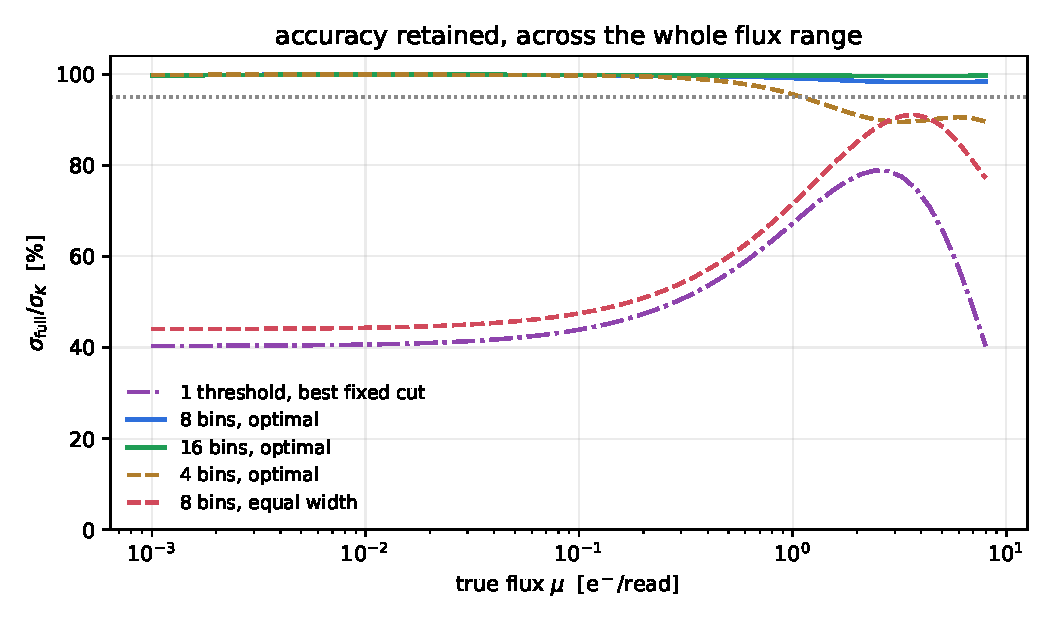
\includegraphics[width=0.85\textwidth]{figures/bins/fig4_efficiency.pdf}
\caption{Accuracy retained versus true flux, for several designs. Four
optimised bins fail only above $\mu \sim 1\ \eminus$/read; eight are flat at
$98$ to $100\,\%$ throughout. Eight equal-width bins lose more than half the
accuracy at low flux.}
\label{fig:eff}
\end{figure}

\section{Monte-Carlo demonstration}

Everything above is a Fisher-information calculation. It predicts the variance
of an efficient estimator; it does not by itself prove that a real
maximum-likelihood fit to eight bins attains it. Figure~\ref{fig:mc} and
Table~\ref{tab:mc} close that gap with simulated data.

The procedure, implemented in \texttt{demo\_optimal\_bins.py}, is: draw reads
from the exact signal chain (Poisson, then Gamma, then Gaussian, then
saturate); bin the \emph{same} simulated reads under each design, so that no
Monte-Carlo noise enters the comparison between designs; fit $\mu$ by grid
maximum likelihood; and measure the scatter over 1200 independent pixels. The
number of reads per pixel is set inversely to the flux so that every point
rests on a comparable number of detected electrons, roughly 400; with a fixed
read count the low-flux estimator would be visibly discrete and its scatter
would stop meaning what the Cram\'er-Rao bound predicts. The reference is a
881-bin histogram whose efficiency against the exact 1\,\ADU\ calculation is
$0.99999$, so it stands in for ``keep everything''.

\begin{figure}[h]
\centering
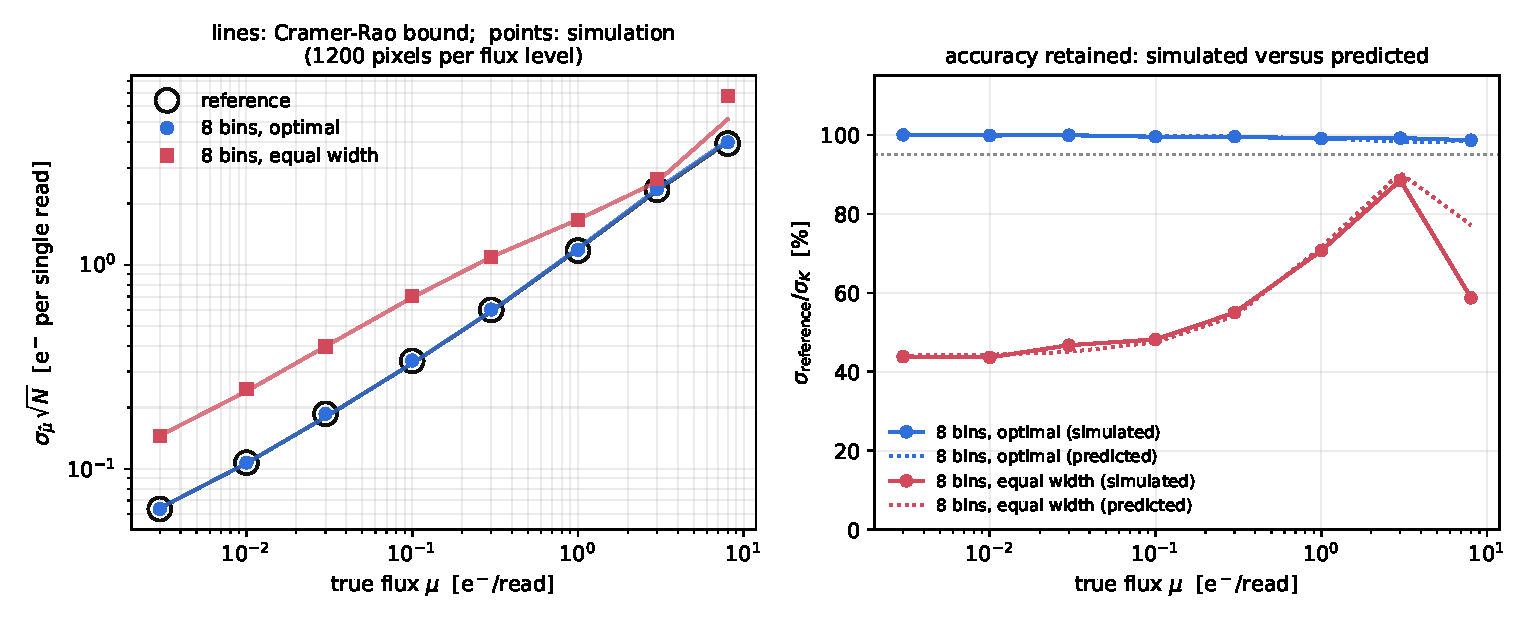
\includegraphics[width=\textwidth]{figures/bins/fig5_montecarlo.pdf}
\caption{Left: simulated scatter of the flux estimate, normalised to one read,
against the Cram\'er-Rao bound (lines). The eight-bin points sit on the
reference curve. Right: accuracy retained, simulated against predicted. The
eight-bin design tracks its prediction to better than one percent; equal-width
bins track theirs too, at a much worse level.}
\label{fig:mc}
\end{figure}

\begin{table}[h]
\centering
\small
\caption{Monte-Carlo results, 1200 independent pixels per flux level.
$\sigma_1 = \sigma_{\hat\mu}\sqrt{N}$ is the scatter normalised to a single
read, directly comparable to $1/\sqrt{I(\mu)}$.}
\label{tab:mc}
\begin{tabular}{rrccc c}
\toprule
$\mu$ & $N$ reads & $\sigma_1$ reference & $\sigma_1$ 8 bins & accuracy retained & predicted\\
\midrule
0.003 & 133\,333 & 0.0636 & 0.0635 & 100.0\,\% & 99.9\,\%\\
0.010 &  40\,000 & 0.1073 & 0.1074 &  99.9\,\% & 99.9\,\%\\
0.030 &  13\,333 & 0.1861 & 0.1862 &  99.9\,\% & 99.9\,\%\\
0.100 &   4\,000 & 0.3385 & 0.3400 &  99.6\,\% & 99.8\,\%\\
0.300 &   2\,000 & 0.6019 & 0.6045 &  99.6\,\% & 99.7\,\%\\
1.000 &   2\,000 & 1.1758 & 1.1866 &  99.1\,\% & 99.1\,\%\\
3.000 &   2\,000 & 2.3359 & 2.3542 &  99.2\,\% & 98.3\,\%\\
8.000 &   2\,000 & 3.9387 & 3.9916 &  98.7\,\% & 98.4\,\%\\
\bottomrule
\end{tabular}
\end{table}

The agreement is close throughout: the simulated worst case over the eight flux
levels is $98.7\,\%$ against a predicted $98.3\,\%$, the difference being
consistent with the residual Monte-Carlo scatter of the variance estimate
(about $2\,\%$ for 1200 trials). The claim in the summary box is therefore not
a theoretical bound alone; a real fit to eight real histograms delivers it.

Over the same simulations, eight equal-width bins retain only $44\,\%$ of the
accuracy at low flux, which is the practical cost of not designing the bins.

\section{Using the code}

\texttt{bin\_optimizer.py} exposes one general-purpose entry point. Give it the
detector and the flux range, and it returns the edges.

\begin{lstlisting}
from bin_optimizer import design_bins

d = design_bins(bias=1000, gain=5000, ron=30, saturation=60000,
                nbins=8, mu_min=1e-3, mu_max=8.0, cic=1e-3)

print(d.summary())          # every cut, in ADU, in u, and in RON sigmas
d.edge_list()               # [0, 1125, 6176, ..., 60000, 60001]
d.worst_accuracy            # 0.9827  -> 98.3 % of the full histogram
d.eta                       # efficiency at each flux in d.mu_grid
\end{lstlisting}

The same thing from the command line, including a scan over $K$:

\begin{lstlisting}
python bin_optimizer.py --bias 1000 --gain 5000 --ron 30 --sat 60000 \
                        --nbins 8 --mu-min 1e-3 --mu-max 8 --cic 1e-3 --scan
\end{lstlisting}

The \texttt{method} keyword selects \texttt{'dp'} (the max-min dynamic
programme), \texttt{'closed'} (the interpretable three-zone family, whose
fitted parameters are returned in \texttt{d.params}), or \texttt{'both'}, the
default, which computes each and keeps whichever wins. \texttt{'closed'} is the
one to use when the edges must be explainable in a paper; the difference in
worst-case $\eta$ is under $0.2\,\%$ at $K=8$.

\texttt{demo\_optimal\_bins.py} regenerates every figure and table in this
document, including the Monte Carlo, in about a minute.

\section{A second detector: large read noise relative to gain}
\label{sec:pesto}

The worked example has $r = \sigma/G = 0.006$: the read-noise peak is a
needle compared with the gain, and one cut serves it. It is worth checking a
detector where that is not true. The PESTO EMCCD at Mont-M\'egantic, whose
constants come from the \texttt{pesto\_stats} MCMC calibration
($b = 303.6178\ \ADU$, $G = 71.060\ \ADU/\eminus$, $\sigma = 6.8164\ \ADU$,
saturation at $5000\ \ADU$), has $r = 0.0959$ and $S = 66.1$, and is used here
over $\mu \in [10^{-3},\,4]\ \eminus$/frame. At $K = 8$:

\begin{center}
\small
\begin{tabular}{rrrrr}
\toprule
bin & lower [\ADU] & upper [\ADU] & $u_{\rm lo}$ & $u_{\rm hi}$\\
\midrule
0 &   0 & 320 & $-4.273$ & 0.231\\
1 & 320 & 331 &  0.231 & 0.385\\
2 & 331 & 404 &  0.385 & 1.412\\
3 & 404 & 492 &  1.412 & 2.651\\
4 & 492 & 601 &  2.651 & 4.184\\
5 & 601 & 740 &  4.184 & 6.140\\
6 & 740 & 949 &  6.140 & 9.081\\
7 & 949 & $\infty$ & 9.081 & $\infty$\\
\bottomrule
\end{tabular}
\end{center}

Worst-case $\eta = 0.9618$, accuracy $98.1\,\%$: eight bins again suffice. But
the design has adapted in two ways that the physics of
Section~\ref{sec:physics} predicts.

First, there are now \emph{two} cuts through the peak, at $+2.40\sigma$ and
$+4.02\sigma$, rather than one. Table~\ref{tab:firstcut} shows why: at
$r = 0.0959$ a single cut at $4\sigma$ would dump $32\,\%$ of all single
electrons into bin~0, and a cut low enough to avoid that would leak read noise.
When neither leak can be made small, the only remedy is to spend a second bin
resolving the overlap region instead of discarding it. The rule of thumb that
emerges is that one cut suffices while $c_1 r \ll 1$, and a second is worth its
bin once $c_1 r \gtrsim 0.2$.

Second, the top cut sits at $u = 9.08$, far below the saturation head-room
$S = 66.1$, and close to $\mu_{\max} + 2.5\sqrt{\mu_{\max}} = 9.0$ for
$\mu_{\max}=4$. With generous head-room, placing the last edge at the physical
saturation level would waste it on a region no read ever reaches.

\subsection{The design this repository ships}
\label{sec:shipped}

Memory is not the binding constraint on this instrument -- a $16 \times 426
\times 1024$ cube of counts is $28\ \mathrm{MB}$ per chunk of frames -- so
\texttt{embin\_config.yaml} ships the $K = 16$ design rather than the $K = 8$
one, and buys back most of the remaining loss:

\begin{center}
\small
\begin{tabular}{lcccccc}
\toprule
$K$ & 4 & 8 & 12 & 16 & 24 & 32\\
\midrule
$\eta$ & 0.8683 & 0.9618 & 0.9815 & \textbf{0.9887} & 0.9940 & 0.9959\\
accuracy & 93.2\,\% & 98.1\,\% & 99.1\,\% & \textbf{99.4\,\%} & 99.7\,\% & 99.8\,\%\\
\bottomrule
\end{tabular}
\end{center}

\noindent The edges, in the convention of \texttt{embin.py} where the final
entry is a formal sentinel for the open top bin:

\begin{lstlisting}
edges: [0, 314, 321, 328, 332, 360, 397, 444, 500, 565,
        640, 725, 819, 922, 1034, 1156, 1157]
\end{lstlisting}

The closed-form family of Section~\ref{sec:opt} wins here, with $m = 3$
peak cuts, $c_{\rm lo} = 1.5$, $c_{\rm hi} = 3.5$, $u_1 = 0.4$ and
$u_{\rm top} = 12.0$: four edges fall inside the read-noise peak, at $+1.52$,
$+2.55$, $+3.58$ and $+4.16\sigma$, and the eleven rungs above it are spaced
uniformly in $\sqrt{u}$ to within $1.6\,\%$ (increments $0.255$ to $0.259$).
Efficiency is flat at $\eta = 0.989$ across the whole flux range, against a
$16$-bin equal-width design which retains only $60\,\%$ of the accuracy at the
sky level of this instrument.

\subsection{On real frames}

Applied to a 1001-frame PESTO sequence (48.97\,ms per frame), cut into fifteen
chunks of 64 frames so that the field's $0.16\ \mathrm{pix\,s^{-1}}$ drift stays
below half a pixel within a chunk, the fitted sky flux is $0.0159$ to
$0.0170\ \eminus$/frame chunk to chunk, against $0.0162 \pm 0.0001$ from the
independent MCMC calibration of the same data: the binning introduces no
detectable bias. Of the $2.79 \times 10^{7}$ pixel values in a chunk, 39 land in
the open top bin, which is the top cut doing exactly what
Section~\ref{sec:physics} asks of it -- sitting where the counts stop, and not
one bin higher.

\section{Scope and caveats}

\begin{itemize}\itemsep3pt
\item The design is optimised for the \emph{worst case} over a stated flux
      range. Widening that range costs accuracy at every flux, so it should be
      set to what the science needs and no wider. Optimising to
      $\mu_{\max} = 1$ instead of $8$ raises the worst-case $\eta$ at $K=8$
      appreciably.

\item Efficiency is measured against the full 1\,\ADU\ histogram, which is the
      correct ceiling for a histogram-based method. It is not a comparison
      against an ideal photon counter: the EM register's own excess noise costs
      information that no binning can recover, and is present in both terms of
      the ratio.

\item The bias, gain and read noise are treated as known. They come from a
      separate calibration; if they are fitted jointly with the flux, the
      relevant object is a Fisher \emph{matrix} and the optimal bins shift,
      generally towards resolving the peak more finely, since that is where
      the bias and read noise are constrained.

\item Bin edges are whole \ADU, because the detector is digitised. The cuts
      through the read-noise peak are rounded \emph{up}, never down: rounding a
      cut down towards the bias admits read-noise leakage, and
      Section~\ref{sec:firstcut} shows how expensive that is. For a detector
      whose read noise is smaller than one \ADU\ the rounding direction alone
      can change $\eta$ from $0.99$ to $0.51$.

\item Clock-induced charge is modelled as an additive Poisson term and is not
      separable from the flux by a single-pixel histogram. The estimator
      returns $\mu$ with $\mu_{\rm CIC}$ already subtracted, on the assumption
      that $\mu_{\rm CIC}$ is known.
\end{itemize}

\bigskip
\noindent\rule{\textwidth}{0.4pt}\\
\footnotesize
References: Basden, A. G., Haniff, C. A., \& Mackay, C. D. 2003, MNRAS, 345,
985. Harps{\o}e, K. B. W., Andersen, M. I., \& Kj{\ae}gaard, P. 2012, A\&A,
537, A50. Daigle, O., Carignan, C., Gach, J.-L., et al. 2009, PASP, 121, 866.

\end{document}
